\begin{tcolorbox}[colback=blue!5!white,colframe=blue!75!black,title=SoMove]
	Software que permite la configuración de dispositivos de variadores de velocidad pertenecientes a la empresa \textbf{Schneider Electric}.
\end{tcolorbox}


\subsubsection{Configuración de parámetros primarios}
Para realizar la configuración del motor se utilizó el software SoMove. Se descargó la ultima versión desde la página oficial de Schneider\footnote{\url{https://www.se.com/ar/es/product-range-presentation/2714-somove/}} y luego, la librería DTM correspondiente al variador a utilizar\footnote{\url{https://www.se.com/ar/es/download/document/Altivar_DTM_Library/}}.

Una vez realizado esto se procedió a generar un nuevo proyecto eligiendo las características del variador (Figura \ref{fig:so1} y \ref{fig:so2}). El próximo paso fue realizar por medio del software la carga de los parámetros del motor (Figura \ref{fig:paramsomove}) y establecer el modo de funcionamiento de las entradas y el protocolo de comunicación.
\begin{figure}[h]
	\centering
	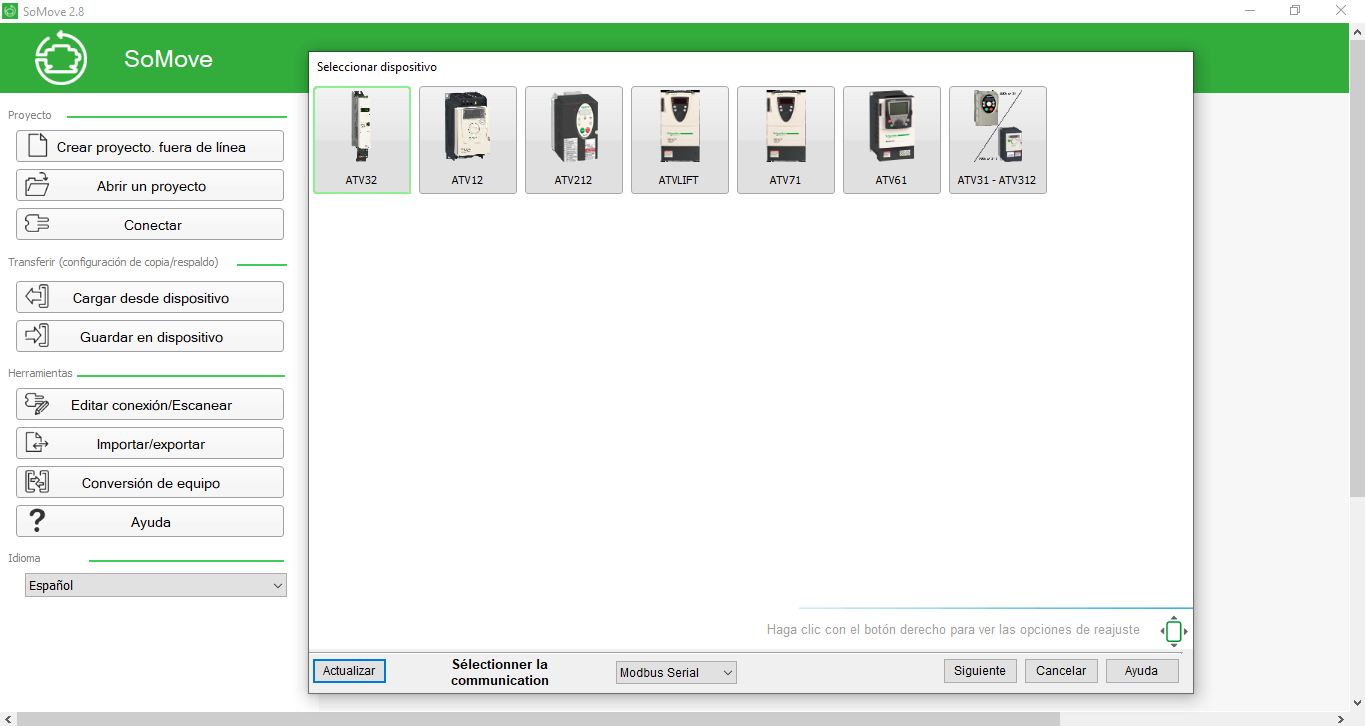
\includegraphics[scale=0.45]{somove1.png}
	\captionof{figure}{Elección de Altivar 312}
	\label{fig:so1}
\end{figure}
\begin{figure}[H]
	\centering
	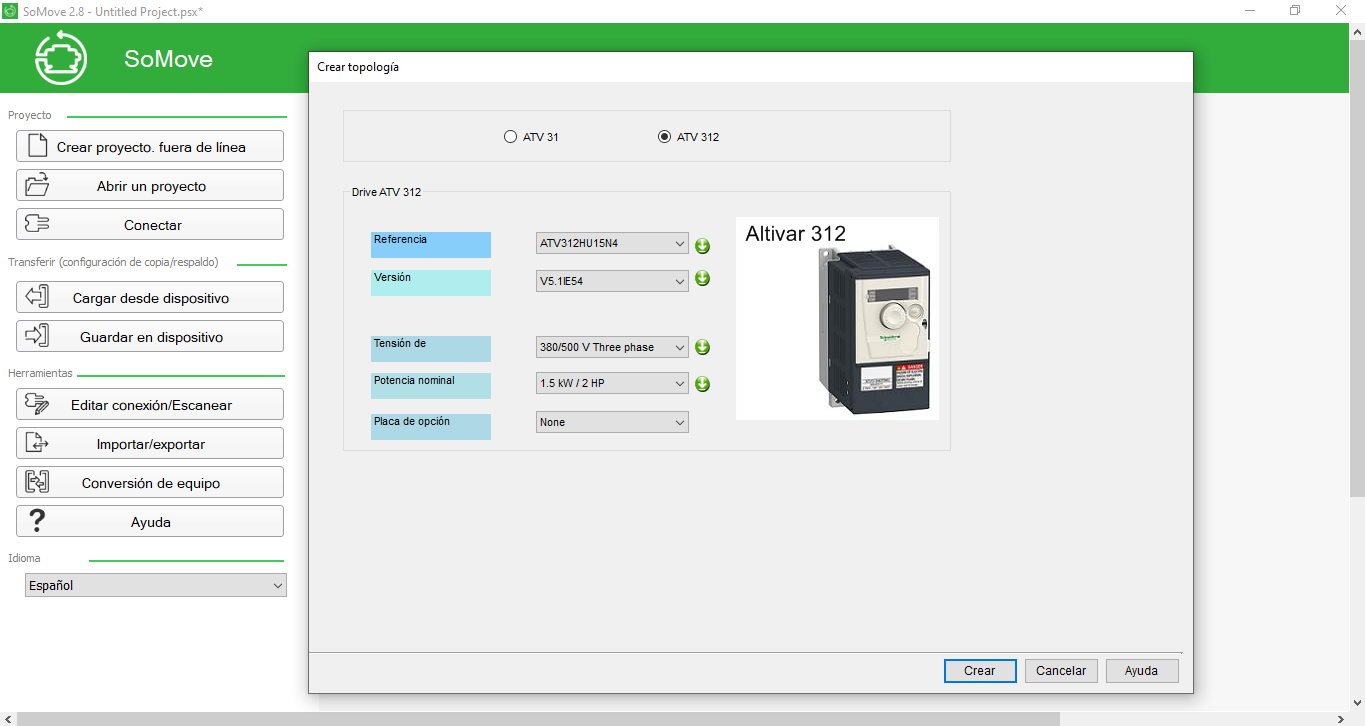
\includegraphics[scale=0.45]{somove2.png}
	\captionof{figure}{Parámetros del variador}
	\label{fig:so2}
\end{figure}

\begin{figure}[H]
	\centering
	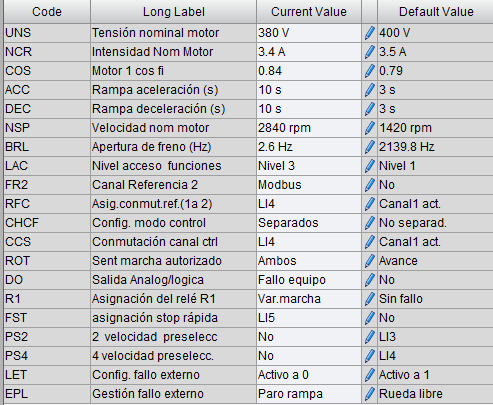
\includegraphics[scale=0.45]{images/paramsomove}
	\caption[Lista de parámetros modificados]{}
	\label{fig:paramsomove}
\end{figure}


Para realizar esta primera configuración se realizó la comunicación de la PC con el variador a través del protocolo \textbf{Modbus} (Figura\ref{fig:pcvar}) a través de un cable realizado por nosotros mismos en la cual en un extremo poseía ficha RJ45 y en el otro un conversor RS485 con ficha USB. Para la construcción de dicho cable fue necesario observar el manual \cite{CANopenMmanual}
\begin{figure}[H]
	\centering
	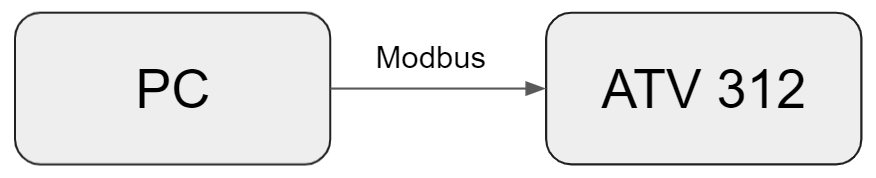
\includegraphics[scale=0.25]{pc_var.png}
	\captionof{figure}{Diegrama comunicación PC- Variador}
	\label{fig:pcvar}
\end{figure}

\begin{figure}
	\centering
	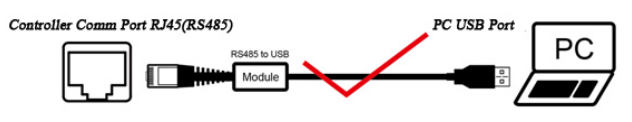
\includegraphics[width=0.7\linewidth]{images/paramsomove1}
	\caption{}
	\label{fig:paramsomove1}
\end{figure}



%Ver si CONFIGURACION DE COMUNICACION CANOPEN VA \hl{capaz que no va acá}
Ver si CONFIGURACION DE COMUNICACION CANOPEN VA \hl{va?}.

